\noindent The Feynman rules demonstrated in the last lecture are specifically for the $\varphi^4$ theory of interacting quantum fields in \textit{position space}, and allow the calculation of $n$-point correlation (Green's) functions, which are not directly observable, but related to scattering amplitudes which are directly observable. We did not rigorously prove, but demonstrated (with $n=2$) the feasibility of and accepted as "definition", that the $n$-point correlation function is equal to the sum of all possible diagrams with $n$ external vertices, subject to the Feynman rules in position space. Keep note that we did not consider $n>2$ or $\lambda>1$ in the following equality.
\begin{align}
G^{(n)}(x_1,\dots,x_n) &= \frac{\bra{0}\mathcal{T}[\hat{\phi}(x_1) \dots \hat{\phi}(x_n)\mathcal{S}]\ket{0}}{\bra{0}\mathcal{S}\ket{0}} \\
&= \left(\text{\small {\stackanchor{sum of all possible diagrams with $n$ external vertices}{subject to Feynman rules in position space}}}\right)
\end{align}

\noindent A ubiquitous issue and deep concern in quantum field theory is the appearance infinities in calculations. Nature seems to suggest that there are no infinities, unless one asks the wrong question. (Are there actually any physical quantities that can be proven to be infinite by experiment, such as the energy levels of the hydrogen atom or the results of continuous scattering theory?) Many infinities that appear due to the application of the Feynman rules will be trivially dispelled (\textit{cf.}, in quantum mechanics when an infinite ground state energy is calculated, simply apply a shift to make it finite). \textbf{Vacuum bubbles} are diagrams with no external vertices (e.g., self interactions) that evaluate to infinity, but will cancel in calculating the $n$-point correlation function $G^{(n)}(x_1,\dots,x_n)$, as we saw in the $n=2$ case in the last lecture.\\

\subsection*{Feynman Rules in Momentum Space ($\varphi^4$ Theory)}

\noindent Remember that the perturbation expansion of the $\mathcal{S}$-matrix and the Green's function can be calculated in momentum space via the Feynman rules in momentum space. The momentum space Feynman propagator has the form
\begin{equation}
\Delta_F(x,y) = \int \frac{d^4 p}{(2\pi)^4} \frac{i e^{-i p \cdot (x-y)}}{p^2-m^2 + i\epsilon}
\end{equation}

\noindent Calculating the perturbation expansion in momentum space may make additional cancellations more apparent. The Feynman rules for $\varphi^4$ theory in momentum space are as follows
\begin{enumerate}
\item For each propagator with momentum $p$, add a factor of $\frac{i}{p^2-m^2+i\epsilon}$.
\item For each (internal) vertex, add a factor of $-i\lambda$.
\item For each external vertex, add a factor of $e^{-ip\cdot x}$.
\item Impose momentum conservation at each vertex.
\item Integrate over undetermined momenta.
\item Divide by symmetry factor.
\end{enumerate}

\begin{figure}[H]
	\centering
	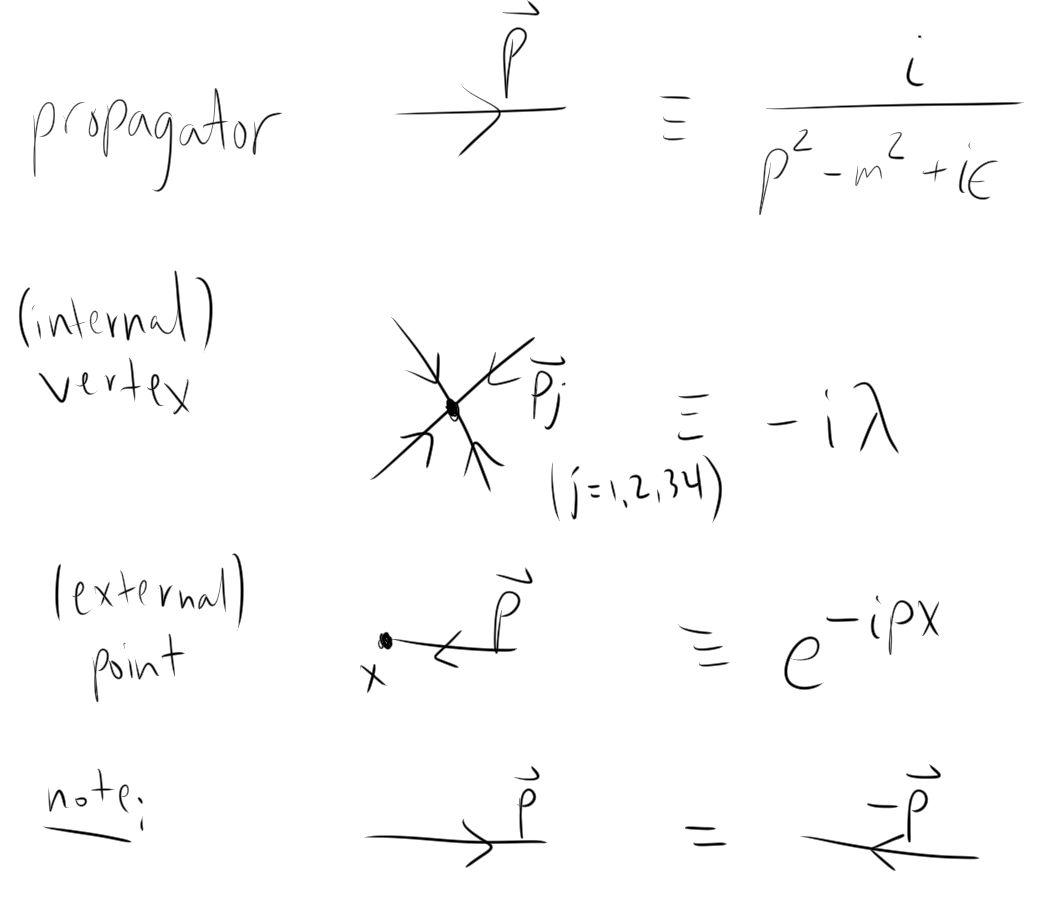
\includegraphics[scale=0.6]{feynmanmom.png}
	\caption{Diagrammatic representation for the Feynman rules in momentum space.}
\end{figure}

\noindent Returning to the $n=2$ case, a general diagram consists of a product of \textit{connected} components and \textit{disconnected} components. Note that the external vertices ($x$ and $y$ in the $n=2$ case) are always connected, since their degrees are odd. For example,

\begin{figure}[H]
	\centering
	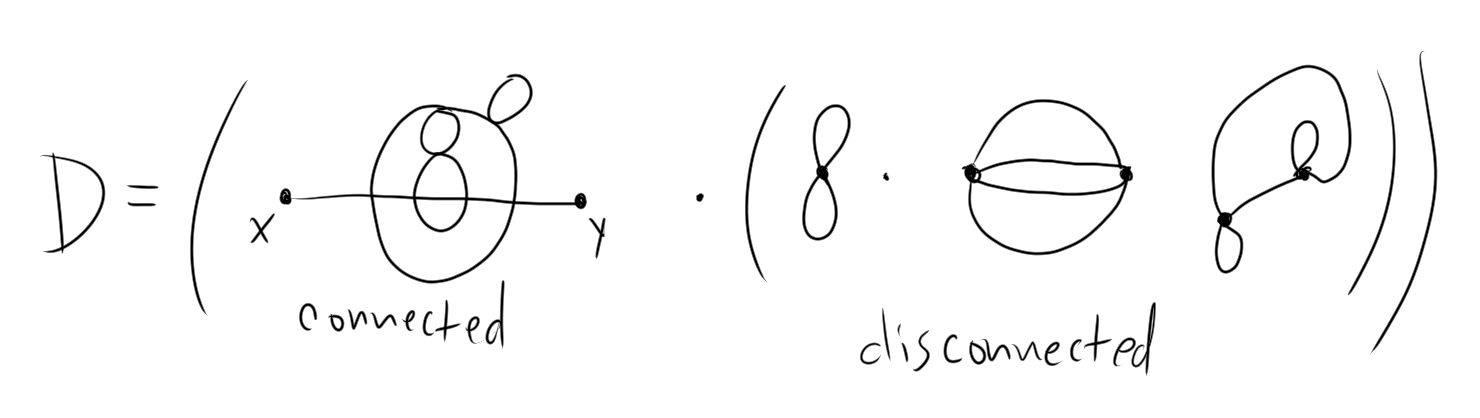
\includegraphics[scale=0.4]{n2diagrams.png}
	\caption{Typical diagram for $n=2$ case.}
\end{figure}

\noindent All possible disconnected pieces form a countable set. 

\begin{figure}[H]
	\centering
	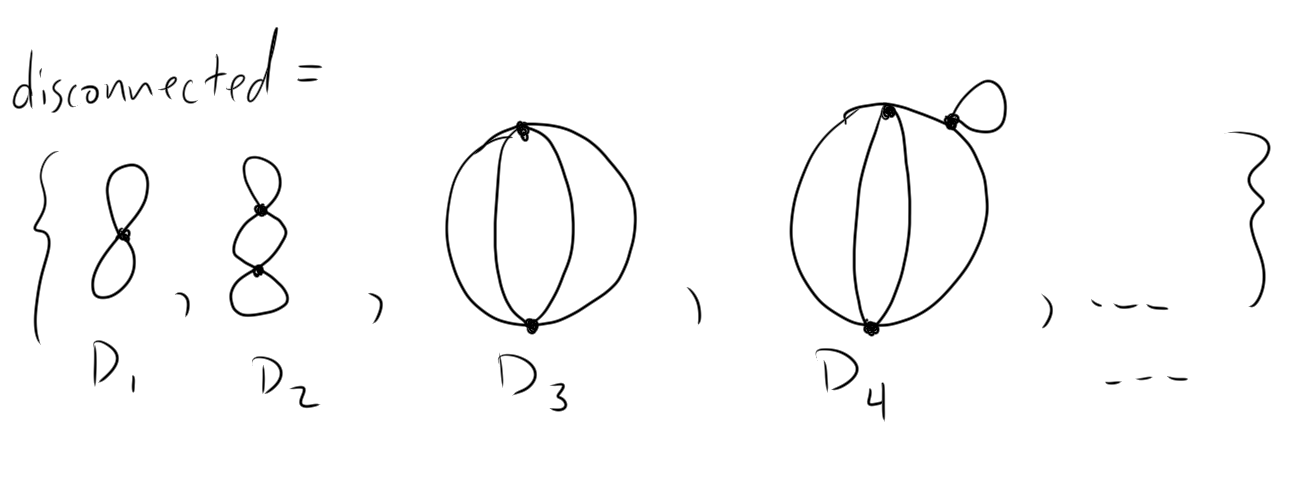
\includegraphics[scale=0.4]{countable.png}
	\caption{Countable set of all possible disconnected pieces.}
\end{figure}

\noindent Each type of disconnected diagram $D_j$ has a unique value $v(D_j)=v_j$, which are all \textit{infinite}. To interpret this result, place a \textbf{cutoff} on the theory. It must be checked that the results, after evaluating the diagrams of the expansion, do not depend on the cutoff imposed. \\

\noindent Suppose that a given diagram $D$ has $n_j$ components of type $D_j$, including the connected component. The value of the diagram is the product of the values of the connected and disconnected components.
\begin{equation}
v_j = v_{connected} \cdot \prod_{j=1}^{\infty} \frac{1}{n_j !} v_j^{n_j}
\end{equation}

\noindent Where $n_j !$ is the symmetry factor. \\

\noindent For the $n=2$ diagram example above, we have the product of the connected piece with disconnected types $D_1$, $D_3$, and $D_2$, respectively, with $n_j=1$ for each diagram type $j$. Therefore the value of the diagram is
\begin{equation}
v(D) = v_{connected} \cdot v_1 \cdot v_3 \cdot v_2
\end{equation}

\begin{figure}[H]
	\centering
	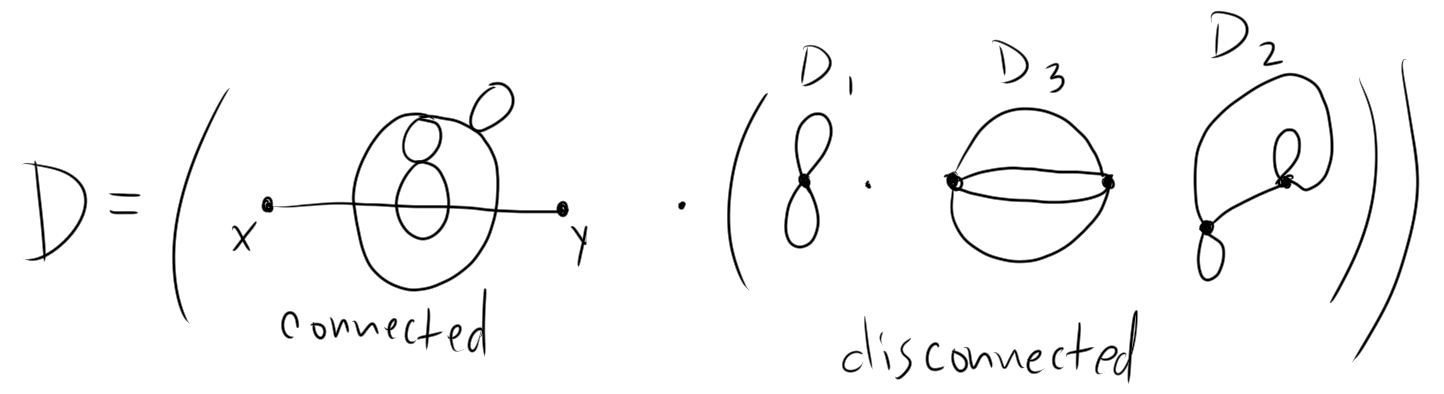
\includegraphics[scale=0.4]{n2diagramslabel.png}
	\caption{Typical diagram for $n=2$ case with disconnected pieces labelled by type.}
\end{figure}

\noindent This allows us to write down a more closed form for the series expansion for $G^{(2)}(x,y)$, and ditch the "all possible diagrams" bit. The numerator of $G^{(2)}(x,y)$ is then
\begin{align}
\text{Numerator(}G^{(2)}(x,y)\text{)} &= \sum_{connected} \sum_{\{n_j\}} v_{connected} \cdot \prod_{j=1}^\infty \frac{1}{n_j !} v_j^{n_j} \\
&= \sum_{conn.} v_{conn.} \sum_{\{n_j\}} \prod_{j=1}^\infty \frac{1}{n_j !} v_j^{n_j} \\
&= \sum_{conn.} v_{conn.} \prod_{j=1}^\infty \sum_{\{n_j\}} \frac{1}{n_j !} v_j^{n_j}  \\
\text{Numerator(}G^{(2)}(x,y)\text{)} &= \sum_{conn.} v_{conn.} \cdot e^{\sum_{j=1}^{\infty} v_j}
\end{align}

\noindent Note that we justify these manipulations of not-necessarily-convergent series by the implemented cutoff, which makes each value finite. Similarly, the denominator is simply the sum over the same exponential
\begin{equation}
\text{Denominator(}G^{(2)}(x,y)\text{)} = e^{\sum_{j=1}^{\infty} v_j}
\end{equation}

\noindent This cancels exactly with the same term in the numerator, pulled out of the sum over connected parts. Therefore, the $2$-point correlation function, which generalizes to $n>2$, is equal to the sum of all connected components subject to the Feynman rules.
\begin{equation}
G^{(2)}(x,y) = \left(\stackanchor{sum over all connected diagrams}{subject to Feynman rules}\right)
\end{equation}

\begin{figure}[H]
	\centering
	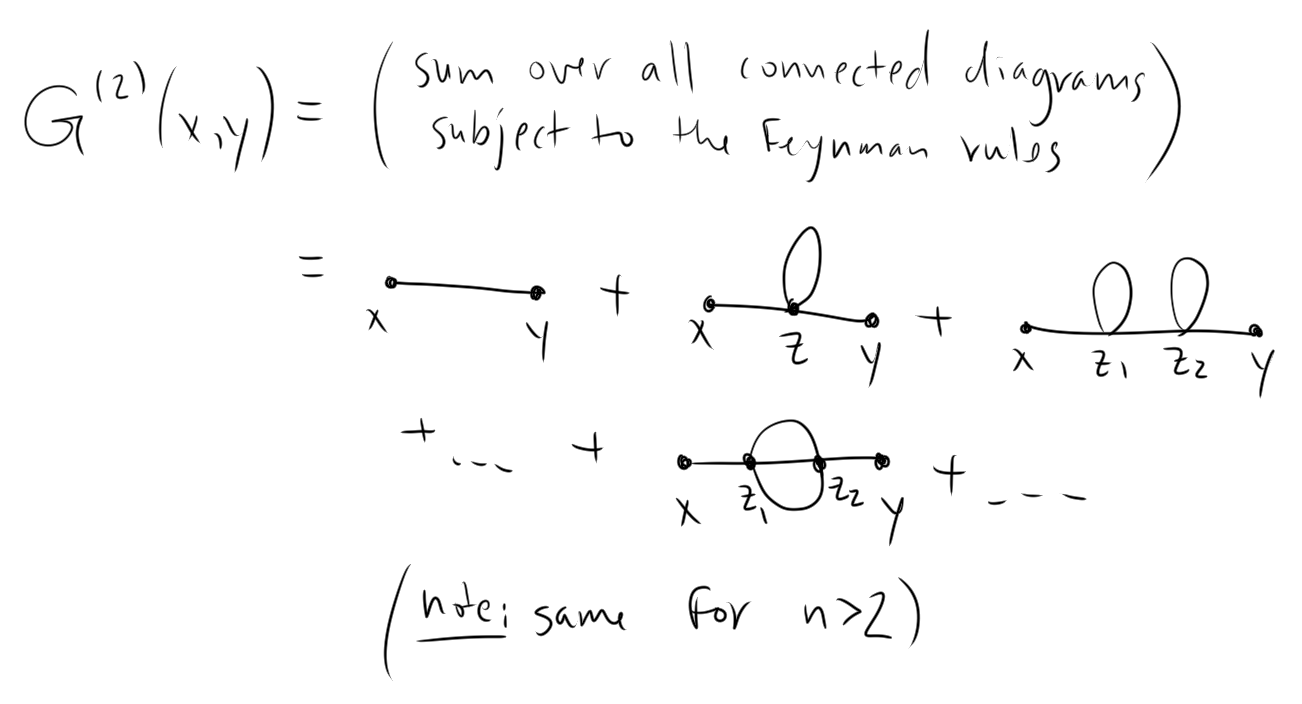
\includegraphics[scale=0.6]{allconnected.png}
	\caption{The sum over all connected diagrams subject to the Feynman rules.}
\end{figure}

\subsection*{Cutoffs in QFT}

\noindent Consider the Klein-Gordon Hamiltonian
\begin{equation}
\hat{H}_{KG} = \frac{1}{2} \int d^3 x \left( \hat{\pi}^2(x) + (\nabla \hat{\phi} (x))^2 + m^2 \hat{\phi}^2(x) \right)
\end{equation}

\noindent This assumes an infinitie number of degrees of freedom, one per each point in spacetime $x \in \mathcal{M}_4$. Now, for example, our theory and understanding of spacetime breaks down below the Planck scale. We can either continue to work in ignorance, or remember that we are dealing in \textit{effective} theories that, hopefully, represent something more fundamental. For example, the Navier-Stokes equation is an effective theory for quantum chromodynamics (QCD). An \textbf{effective theory} is a description which explains all observations up to a given scale $s$, often expressed in inverse length, and may break down beyond the given scale. \\

\noindent To impose a cutoff on the Hamiltonian, add a "fixing" term $\hat{H}_\Lambda$ which is well-behaved up to the scale $\Lambda$, and must match predictions of the original Hamiltonian $\hat{H}$
\begin{equation}
\hat{H} \to \hat{H}' = \hat{H} + \hat{H}_\Lambda
\end{equation}

\noindent To modify the new Hamitonian for other scales, Wilson's \textbf{renormalization theory} may be used, where the "fixing" Hamiltonian $\hat{H}_\Lambda$ is parameterized by the field operators and their derivatives
\begin{align}
\hat{H}_\Lambda &= \sum_{polynomials} \mathcal{P}(\hat{\phi}, \nabla \hat{\phi}, \nabla^2 \hat{\phi}, \dots, \hat{\pi}, \nabla \hat{\pi}, \nabla^2 \hat{\pi}, \dots) \\
&= c_0 \hat{\phi} + c_1 \hat{\phi}^2 + \dots + d_0 \hat{\pi} + d_1 \hat{\pi}^2 + \dots + e_1 (\nabla \hat{\phi})^2 + \dots
\end{align}

\noindent Only a finite number of the coefficients are nonzero and have an effect on observations beyond the scale $\Lambda$. By effect, the value of the term in the sum over field operator polynomials is not suppressed by inverse powers of $\Lambda$. Such terms that are not suppressed and have an effect on observations are called \textbf{relevant terms}. Any cutoff that is imposed must differ only by relevant terms. \\

\noindent For example, the relevant terms up to 4 dimensions is 
\begin{equation}
\{ \hat{\phi}, \hat{\phi}^2, \nabla^2 \hat{\phi}, \hat{\pi}, \hat{\pi}^2, \hat{\phi}^3, \hat{\phi}^4 \}.
\end{equation}

\noindent The simplest cutoff to impose on the momentum states of the free Klein-Gordon Hamiltonian is
\begin{equation}
\hat{H}_{KG} = \int \frac{d^3 p}{(2\pi)^3} \omega_p \hat{a}_p^\dagger \hat{a}_p \to \hat{H}_{KG}+\hat{H}_\Lambda = \int_{|p|<\Lambda} \frac{d^3 p}{(2\pi)^3} \omega_p \hat{a}_p^\dagger \hat{a}_p
\end{equation}

\noindent And the simplest cutoff for $\varphi^4$ interaction is
\begin{equation}
\hat{H}_{\varphi^4} = \frac{\lambda}{4 !} \int d^3 x \, \hat{\phi}^4(x) \to \hat{H}_{\varphi^4} + \hat{H}_\Lambda = \int_{|p_j|<\Lambda} d^3 p_1 d^3 p_2 d^3 p_3 d^3 p_4 (\dots)
\end{equation}

\noindent The new Hamiltonian for the quantum Klein-Gordon field with $\varphi^4$ interactions, and an imposed cutoff at scale $\Lambda$ is then written as
\begin{align}
\hat{H} \to \hat{H'} &= \hat{H}_{KG} + \hat{H}_{\varphi^4} + \hat{H}_\Lambda \\
&= \int_{|p|<\Lambda} \frac{d^3 p}{(2\pi)^3} \omega_p \hat{a}_p^\dagger \hat{a}_p + \int_{|p_j|<\Lambda} d^3 p_1 d^3 p_2 d^3 p_3 d^3 p_4 (\dots)
\end{align}